% Chapter 3

\chapter{\uppercase{System Design}} % Main chapter title
\label{ch:chap3} % For referencing
\begin{spacing}{1.5} 
\begin{sloppypar}
There are 3 workflow for creating an Autonomous Driving Agent using this project
\begin{itemize}
    \item Data collection and annotation
    \item Building Vector Database
    \item Autonomous Driving Environment Interaction Loop
\end{itemize}

\begin{figure}[h]
\begin{center}
\includegraphics[scale=0.5]{3/duckieTown.png}
\caption{DuckieTown}
\label{fig:DuckieTown}
\end{center}
\end{figure}

% \subsection{4way}


\begin{sidewaysfigure}[h]
\begin{center}
\includegraphics[scale=0.28]{3/retrieval_rag.png}
\caption{RAG Retrieval Architecture}
\label{fig:archi}
\end{center}
\end{sidewaysfigure}

\begin{sidewaysfigure}[h]
\begin{center}
\includegraphics[scale=0.28]{3/rag generation.png}
\caption{RAG Generation Architecture}
\label{fig:rag_generation}
\end{center}
\end{sidewaysfigure}



\section{DATA COLLECTION TOOL}
The Data Collection tool module consists of 2 sub-modules. 
Data collection tools are indispensable in the realm of research and analysis, serving as the backbone for acquiring accurate and reliable data. These tools facilitate a systematic approach to gathering information, ensuring consistency and reducing biases that could compromise the integrity of the data. The significance of these tools extends across various domains, from business intelligence to scientific research, where they enable the extraction of meaningful insights from raw data. 

In the digital age, data collection tools have evolved to handle the vast amounts of information generated every second. They range from simple online surveys to complex analytics software, each designed to fulfill specific research needs. For instance, surveys are commonly used to collect quantitative data, while interviews and focus groups are tailored for qualitative insights. 

Moreover, the importance of data collection tools lies in their ability to transform disparate data points into coherent patterns and trends. This transformation is crucial for making informed decisions, developing strategies, and predicting future trends. In business, for example, data collection tools can reveal consumer behavior patterns, market trends, and operational inefficiencies, guiding strategic planning and competitive positioning.

In healthcare, data collection tools are used to track patient outcomes, improve treatment protocols, and manage public health initiatives. In education, they assist in evaluating student performance, curriculum effectiveness, and institutional policies. Similarly, in government, these tools support policy development, resource allocation, and service delivery.

The advent of big data and advanced analytics has further underscored the importance of robust data collection tools. They now must not only collect data but also ensure its quality, relevance, and timeliness. With the integration of artificial intelligence and machine learning, data collection tools are becoming smarter, capable of identifying patterns and anomalies that would otherwise go unnoticed.

In conclusion, data collection tools are vital for capturing the essence of the complex world around us. They empower researchers, analysts, and decision-makers with the clarity needed to navigate the intricacies of their respective fields. As we continue to advance technologically, the development and refinement of these tools will remain a critical focus, ensuring that our decisions are grounded in solid, empirical evidence.

\subsection{Recorder}
The data collection tool's recorder is used to procure the dataset required by the Autonomous Driving agent. The Data Collection tool captures small clips from a specific window. You can specific the window, the number of frames per second you are recording and number of frames per clip. You can run this data collection tool in the background and record the particular actions you perform.
\subsection{Data Annotation Tool}
The data annotation tool is used to annotate the recorded clips for the Autonomous Driving agent to use. This is required because the Autonomous Driving agent uses both textual and visual data to understand the semantic meaning of the visual data.

    


\section{RETRIEVAL AUGMENTED GENERATION}

Retrieval-Augmented Generation (RAG) represents a significant advancement in the field of natural language processing (NLP) and Artificial Intelligence (AI). It is a hybrid approach that combines the strengths of two distinct models: retrieval-based and generative. The retrieval component of RAG is responsible for sourcing relevant information from a vast knowledge base, which can include structured databases or unstructured text. This process ensures that the data used for generating responses is grounded in factual and authoritative content, thereby enhancing the reliability and accuracy of the output.

The generative component of RAG then takes this retrieved information and constructs coherent and contextually relevant text. This could be in the form of answers to questions, dialogue for chatbots, or even content for articles. By integrating these two components, RAG effectively addresses some of the limitations inherent in purely generative models, such as the production of outdated or inaccurate information, and the potential for bias and misinformation.

One of the key benefits of RAG is its ability to remain current and specific without the need for constant retraining of the model. This is particularly advantageous for applications requiring up-to-date information or domain-specific knowledge. Additionally, RAG can significantly reduce the computational and financial costs associated with training large language models (LLMs), as it leverages existing knowledge bases rather than relying solely on the data it was trained on.

In practical terms, RAG can be utilized across a wide range of NLP tasks. For instance, in an AI chatbot designed to provide medical information, RAG can retrieve the latest research and guidelines from medical databases to inform its responses, ensuring that users receive the most current and accurate information. Similarly, in content generation, RAG can pull from recent news articles or scientific papers to create content that is both informative and timely.

Moreover, RAG's flexibility allows it to adapt to various languages and domains, making it a versatile tool for global applications. Its architecture, which augments the capabilities of LLMs by adding an information retrieval system, provides developers with greater control over the generated text output. This control is crucial for maintaining the quality and trustworthiness of AI-generated content.

In conclusion, Retrieval-Augmented Generation is a transformative technology that enhances the capabilities of AI in understanding and generating human language. By combining retrieval and generation, RAG offers a more accurate, relevant, and versatile solution for a multitude of NLP applications, pushing the boundaries of what is possible in the realm of AI and machine learning.



To implement RAG, we need a Vector Store. This Vector Store must have efficient lookup time to find the top k similar context information. Algorithms like K-Nearest Neighbors can be employed here. In our Autonomous Driving agent, we go for a simple linear search for finding the top k similar clips. This is because we currently only have a small amount of data, so for this scenario highly efficient algorithms are not necessary. Moving forward, we will be implementing a more efficient and scalable vector database.


\section{TEXT GENERATION}



Text generation using Large Language Models (LLMs) represents a significant advancement in the field of natural language processing (NLP). These models, trained on vast datasets, have the ability to generate coherent and contextually relevant text that closely mimics human writing. The underlying architecture of LLMs, such as the Transformer model, enables them to capture the nuances of language through deep learning techniques. They utilize mechanisms like attention and context to generate text that is not only grammatically correct but also semantically rich.

The training process of LLMs involves unsupervised learning, where the model is exposed to large corpora of text and learns to predict the next word in a sequence, thereby understanding language patterns and structures. This process equips LLMs with a broad understanding of language, enabling them to perform a variety of tasks such as translation, summarization, and question-answering. Moreover, the adaptability of LLMs allows for fine-tuning on specific domains or styles, enhancing their versatility.

One of the most remarkable aspects of LLMs is their ability to generate creative content. Whether it's composing poetry, writing stories, or even creating code, LLMs can produce original content that often requires a second glance to distinguish from that written by humans. This capability has opened up new possibilities in content creation, where LLMs can assist in drafting articles, generating dialogue for characters in games, or providing educational content.

However, the use of LLMs also raises important ethical considerations. The potential for generating misleading information or biased content is a concern that developers and users must address. Ensuring that LLMs are used responsibly involves incorporating checks and balances to prevent the dissemination of harmful content. Additionally, the environmental impact of training and running these large models is a subject of ongoing discussion, prompting a search for more efficient and sustainable methods.

In conclusion, text generation using LLMs is a rapidly evolving technology with immense potential. Its applications span across various industries, revolutionizing the way we interact with and produce written content. As the technology continues to advance, it will be crucial to navigate the challenges it presents to maximize its benefits for society.

There are many methods to save and load models. Recent popular format for saving and loading LLMs is called GGUF. With GGUF, you do not need to load the tokenizer, embedding layer and transformer seperately. Instead, all of it is saved as a single file. GGUF format is most popular to save quantized Large Language Models.

\section{VISION ENCODER}

The vision encoder must be able to understand spatio temporal context information between the sequence of frames. These encoded values must then by aligned with the embedding of description of the video. This alignment is necessary as the final embeddings  of the vision encoder along with prompt embeddings are used as query to find the top k similar clips in the RAG methodology.  

The vision transformer cannot get the entire sequence of image as input. It has to be split into patches. Then encoded with patch encoding and positional encoding. 

The Video Swin Transformer represents a significant advancement in the field of computer vision, particularly in the encoding of video data. It is a model that builds upon the Swin Transformer architecture, which is designed for image domain, to effectively handle video inputs. The key innovation of the Video Swin Transformer lies in its ability to capture the temporal dynamics of video data, which is crucial for tasks such as action recognition and scene understanding.

In mathematical terms, the Video Swin Transformer operates on 3D patches extracted from the input video. These patches are then processed through a series of Transformer layers that model the relationships between different patches. The Transformer layers use self-attention mechanisms, which can be represented mathematically as:

$$
\text{Attention}(Q, K, V) = \text{softmax}\left(\frac{QK^T}{\sqrt{d_k}}\right)V
$$

Here, \( Q \), \( K \), and \( V \) represent the query, key, and value matrices, respectively, which are derived from the input patches. The term \( d_k \) denotes the dimensionality of the key vectors, and the softmax function is applied to the rows of the matrix resulting from \( QK^T \).

The Video Swin Transformer introduces a hierarchical structure that allows it to handle the large-scale nature of video data efficiently. This is achieved by partitioning the video into non-overlapping 3D patches and then applying self-attention within local windows. As the layers go deeper, the windows are merged hierarchically, increasing the receptive field and enabling the model to capture more global information. The hierarchical nature of the model can be expressed as:

$$
\text{Swin}(x) = \text{W-MSA}(\text{LN}(x)) + x
$$

$$
\text{Swin}(x) = \text{SW-MSA}(\text{LN}(\text{Swin}(x))) + \text{Swin}(x)
$$

In the above equations, \( \text{W-MSA} \) and \( \text{SW-MSA} \) refer to the window-based multi-head self-attention and shifted window multi-head self-attention operations, respectively. \( \text{LN} \) denotes layer normalization, and \( x \) is the input to the respective layer.

The adaptability of the Swin Transformer to video tasks is further enhanced by its ability to leverage pre-trained image models, which provides a rich initialization that benefits video understanding. The Video Swin Transformer has demonstrated state-of-the-art performance on various video recognition benchmarks, making it a powerful tool for video analysis applications.


The patch encoding is converting a patch into a linear array. Patch encoding in vision transformers is a pivotal step in processing images for machine learning tasks. It involves the division of an image into fixed-size patches and then encoding these patches into a latent space that can be used for further processing by the transformer model. Mathematically, this process can be represented as follows: given an image \( X \in \mathbb{R}^{H \times W \times C} \), where \( H \), \( W \), and \( C \) represent the height, width, and number of channels of the image respectively, the image is divided into \( N \) patches each of size \( P \times P \times C \). Each patch is then flattened into a vector of size \( P^2 \times C \), and these vectors are linearly projected into a \( D \)-dimensional space using a trainable embedding matrix \( E \in \mathbb{R}^{(P^2 \cdot C) \times D} \). The mathematical formula for this encoding is \( z = E \cdot \text{vec}(x_p) \), where \( x_p \) is the flattened patch vector and \( z \) is the resulting encoded patch vector.

This encoding process is crucial because it allows the model to handle images of varying sizes and reduces the computational complexity compared to processing the entire image at once. The encoded patches are then fed into the transformer encoder, which uses self-attention mechanisms to capture the global dependencies between patches. The positional information of each patch is also important, as it helps the model to understand the spatial structure of the image. This is often incorporated through positional encodings that are added to the patch encodings before they are input to the transformer model.

The use of patch encoding in vision transformers represents a significant shift from the traditional Convolutional Neural Networks (CNNs) that dominated image processing tasks. Unlike CNNs, which apply filters to overlapping regions of the image, patch encoding treats each patch independently until the self-attention mechanism in the transformer model allows for interaction between them. This approach has shown great promise in various computer vision tasks, offering a more flexible and powerful way to model the complex relationships present in visual data. The mathematical rigor and the ability to capture long-range dependencies make vision transformers, powered by patch encoding, a cutting-edge tool in the field of machine learning and artificial intelligence.


The positional encoding is just to ensure that each position is differentiable by the transformer. This is down by concatenating a small random number to each of the patch encoding. 
Positional encoding plays a crucial role in vision encoding, particularly in the context of neural networks that deal with sequential data. In the absence of inherent sequential information within the input data, positional encodings are used to provide the model with the notion of the order of the elements. This is particularly important in models like Transformers, which, unlike RNNs, do not process data in sequence. The mathematical formulation of positional encoding typically involves a set of functions that map a position in the sequence to a high-dimensional space of real numbers. For instance, in the Transformer model, the positional encoding is added to the input embeddings at the bottom of the model architecture. The functions used for this purpose are often sinusoidal, as they can allow the model to easily learn to attend by relative positions, due to the fact that for any fixed offset \( k \), \( \sin(x+k) \) and \( \cos(x+k) \) can be represented as a linear function of \( \sin(x) \) and \( \cos(x) \). The standard positional encoding formula in a Transformer is given by:

$$
PE_{(pos,2i)} = \sin\left(\frac{pos}{10000^{2i/d_{model}}}\right)
$$

$$
PE_{(pos,2i+1)} = \cos\left(\frac{pos}{10000^{2i/d_{model}}}\right)
$$

where \( pos \) is the position, \( i \) is the dimension, and \( d_{model} \) is the dimensionality of the model's output space. This encoding can be extended to two-dimensional space, which is particularly useful for vision tasks. In this case, the positional encoding would take into account both the x and y coordinates of the position in the image. The 2D positional encoding can be formulated as:

$$
PE_{(x,y,2i)} = \sin\left(\frac{x}{10000^{2i/d_{model}}} + \frac{y}{10000^{2i/d_{model}}}\right)
$$

$$
PE_{(x,y,2i+1)} = \cos\left(\frac{x}{10000^{2i/d_{model}}} + \frac{y}{10000^{2i/d_{model}}}\right)
$$

This approach allows the model to understand the relative positioning of features in an image, which is essential for tasks such as image recognition, segmentation, and object detection. The use of positional encoding in vision encoding ensures that spatial hierarchies and relationships between different parts of the image are maintained and understood by the neural network, leading to more accurate and effective models for visual data processing.

The pre-trained vision transformer must have been trained with modality used in our work, i.e video without audio. This is to ensure that vision transformer produces useful and meaningful outputs. 

The output embedding from the vision transformer is then passed through Multi-Layered Perceptron. The purpose of this MLP is to take the vision transformer output and transform it into the embeddings of the video description embeddings. By doing this, we have built a vision encoder that takes 3 frames input and returns embedding vector that is close to the embedding vector that represents the video description. 

The alignment head is MLP with GELU activation function.

A Multi-Layer Perceptron (MLP) is a class of feedforward artificial neural network (ANN) that consists of at least three layers of nodes: an input layer, a hidden layer, and an output layer. Except for the input nodes, each node is a neuron that uses a nonlinear activation function. MLP utilizes a supervised learning technique called backpropagation for training. 

The nodes of the intermediate or hidden layers typically use a sigmoid function as their activation function, represented by the formula $$\sigma(x) = \frac{1}{1 + e^{-x}}$$ where \(x\) is the input to a neuron. This function introduces non-linearity to the model, allowing the network to learn more complex tasks.

For a given input vector \(X\), the output \(Y\) of a neuron is calculated using the weighted sum of the inputs, including a bias term, followed by an activation function. This can be represented as $$Y = \sigma(\sum_{i=1}^{n} w_i x_i + b)$$ where \(w_i\) represents the weight associated with the \(i\)-th input \(x_i\), and \(b\) is the bias.

The learning process involves adjusting these weights and biases to minimize the error in predictions. The error is quantified using a loss function, such as the mean squared error for regression tasks, given by $$E = \frac{1}{2}\sum_{i=1}^{n} (y_i - \hat{y}_i)^2$$ where \(y_i\) is the true value and \(\hat{y}_i\) is the predicted value by the model.

During backpropagation, the derivative of the error with respect to the weights is computed to update the weights in the direction that minimizes the error. This involves calculating the gradient of the loss function, which, for the mean squared error and sigmoid activation, can be expressed as $$\frac{\partial E}{\partial w_i} = (y_i - \hat{y}_i) \cdot \sigma'(\hat{y}_i) \cdot x_i$$ where \(\sigma'(\hat{y}_i)\) is the derivative of the activation function.

MLPs are widely used for pattern recognition, classification, and regression tasks. Their ability to model complex non-linear relationships makes them powerful tools in the field of machine learning. However, they can be prone to overfitting and may require techniques such as regularization and dropout to generalize better to unseen data. Despite these challenges, MLPs remain a fundamental building block in the architecture of deep learning models.

The Gaussian Error Linear Unit (GELU) is a type of activation function that is used in the field of neural networks, particularly in deep learning models. It combines properties of both the rectified linear unit (ReLU) and the normal distribution function, which allows it to model complex functions more effectively than traditional activation functions. The GELU function is defined mathematically as:

$$ GELU(x) = x \cdot \Phi(x) $$

where \( x \) is the input to the activation function, and \( \Phi(x) \) is the cumulative distribution function of the standard normal distribution. The formula for \( \Phi(x) \) is given by:

$$ \Phi(x) = \frac{1}{2} \left[1 + \text{erf}\left(\frac{x}{\sqrt{2}}\right)\right] $$

Here, \( \text{erf} \) represents the Gauss error function, which is a non-elementary function that cannot be expressed in terms of elementary functions. It is defined as:

$$ \text{erf}(x) = \frac{2}{\sqrt{\pi}} \int_{0}^{x} e^{-t^2} dt $$

The GELU activation function has been found to perform well in practice and is particularly useful in transformer models, such as those used in natural language processing tasks. It allows the network to learn to make more nuanced decisions about when to activate neurons, leading to improved model performance on a variety of tasks. The GELU function is smoothly non-linear when \( x \) is small, and approximately linear when \( x \) is large, which helps to mitigate the vanishing gradient problem that can occur with other activation functions like the sigmoid or hyperbolic tangent functions. This characteristic makes GELU an attractive choice for researchers and practitioners in the field of machine learning.



\begin{figure}[h]
\begin{center}
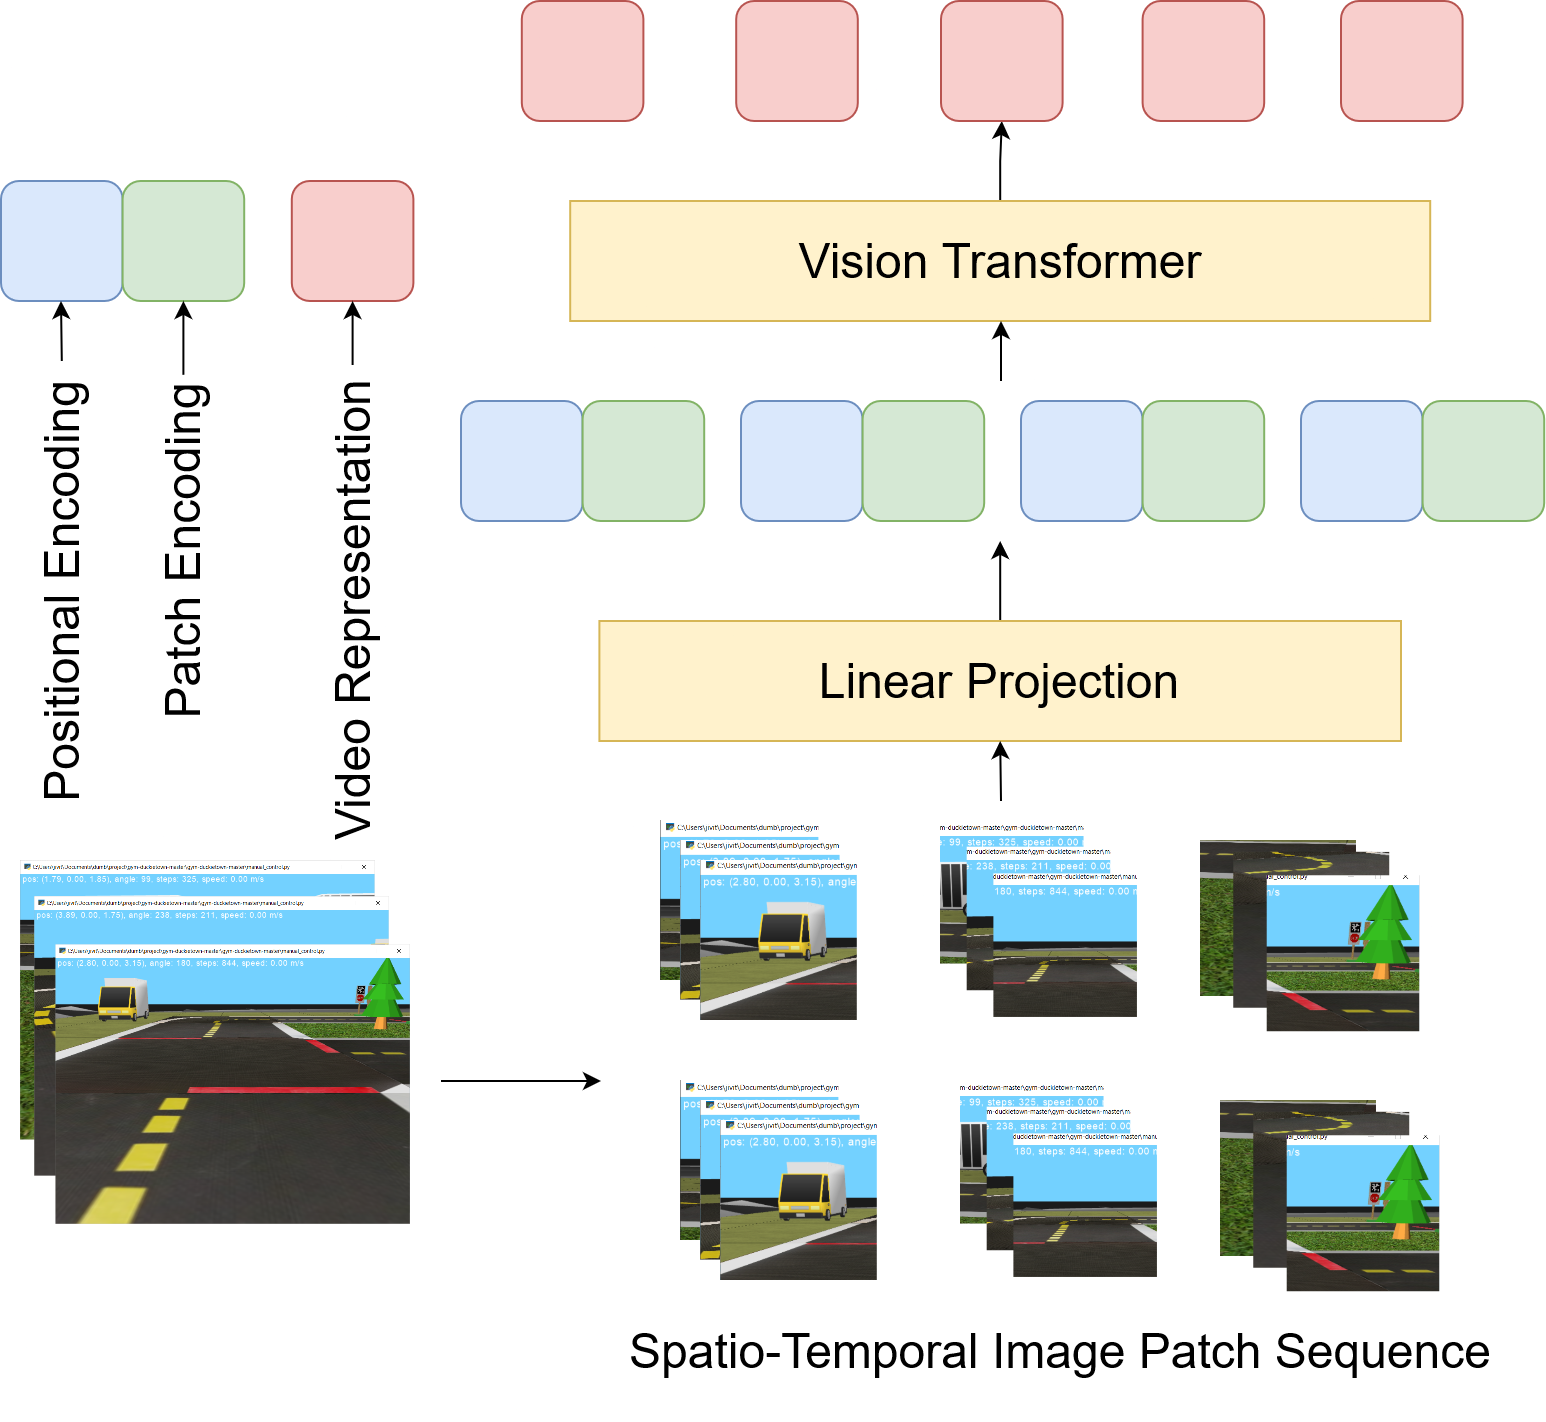
\includegraphics[scale=0.26]{3/Dissertation II_Video_Encoder.png}
\caption{Video Encoder}
\label{fig:Video Encoder}
\end{center}
\end{figure}

\begin{figure}[h]
\begin{center}
\includegraphics[scale=0.5]{3/Data Annotation.png}
\caption{Dataset Annotator}
\label{fig:Dataset Annotator}
\end{center}
\end{figure}
\end{sloppypar}
 \end{spacing}

 